%\documentclass[useAMS,referee, usegraphicx]{biom}
\documentclass[useAMS,referee,usenatbib]{biom}
%\documentclass[useAMS, usegraphicx]{biom}
\usepackage{amsmath}
\usepackage[pdftex]{graphicx}
\usepackage{url}


%%%%% PLACE YOUR OWN MACROS HERE %%%%%

\def\bSig\mathbf{\Sigma}
\newcommand{\VS}{V\&S}
\newcommand{\tr}{\mbox{tr}}

\title[Mixture model detection functions]{Mixture models for distance sampling detection functions}

\author{David L. Miller$^{*}$\email{dave@ninepointeightone.net}, Len Thomas\\
Centre for Research into Ecological and Environmental Modelling,\\
University of St Andrews, St Andrews KY16 9LZ, Scotland}

\begin{document}
\label{firstpage}

\begin{abstract}
This version: \today %Remove this before submitting!

*** 15 lines or 225 words max ***

We present a new class of models for the detection function in distance sampling surveys of wildlife populations, based on finite mixtures of simple parametric key functions such as the half-normal. The models share many of the features of the widely-used ``key function plus series expansion'' formulation: they are flexible, produce plausible shapes with a small number of parameters, allow incorporation of covariates in addition to distance and can be fitted using maximum likelihood. One advantage over current methods is the mixtures are automatically monotonic non-increasing and non-negative, so constrained optimization is not required to ensure distance sampling assumptions are met. The mixture formulation is compared to existing methods using extensive simulations and case studies on real data. *** Need to put a summary of what we find here (better at dealing with spikes -- say that's another advantage?) ***
\end{abstract}

\begin{keywords}
Continuous mixture; Finite mixture; Line transect sampling; Monotonicity constraints; Multiple covariate distance sampling; Point transect sampling.
\end{keywords}

\maketitle


%  If you are using the referee option, a new page, numbered page 1, will
%  start after the summary and keywords.  The page numbers thus count the
%  number of pages of your manuscript in the preferred submission style.
%  Remember, ``Normally, regular papers exceeding 25 pages and Reader Reaction 
%  papers exceeding 12 pages in (the preferred style) will be returned to 
%  the authors without review. The page limit includes acknowledgements, 
%  references, and appendices, but not tables and figures. The page count does 
%  not include the title page and abstract. A maximum of six (6) tables or 
%  figures combined is often required.''

%  You may now place the substance of your manuscript here.  Please use
%  the \section, \subsection, etc commands as described in the user guide.
%  Please use \label and \ref commands to cross-reference sections, equations,
%  tables, figures, etc.
%
%  Please DO NOT attempt to reformat the style of equation numbering!
%  For that matter, please do not attempt to redefine anything!

\section{Introduction}
\label{s:intro}


Distance sampling \citep{Buckland:2001vm,Buckland:2004ts} is a suite of methods for estimating the size or density of biological populations.  There are two main variants: line and point transects. In both, an observer visits a randomly-located set of transect lines or points and records the distance, $y$, from the transect to each object of interest (i.e., animals or plants of the target species) that is detected within some truncation distance $w$.  Not all objects within $w$ are assumed to be detected; instead the observed distances are used to estimate the parameters, $\bm{\theta}$, of a detection function model, $g(y;\bm{\theta})$, which describes how the probability of detection declines with increasing distance.  An assumption of the basic method is that $g(0;\bm{\theta})=1$. Given estimates of $\bm{\theta}$, it is straightforward to estimate population size or density (see Section \ref{s:popsize}).

A key part of distance sampling, therefore, is specification of the detection function model.  \citet[][Chapter 2]{Buckland:2001vm} provide a set of criteria for judging the utility of candidate model classes. Detection function models should be:
\begin{enumerate}
\item flexible, so that they can take a wide variety of shapes;
\item efficient, in the sense that many plausible shapes can be represented using few parameters;
\item flat at zero distance (i.e., $g'(0;\bm{\theta})=0$), indicating that object in the immediate vicinity of the observer are equally detectable; and,
\item monotonic non-increasing with increasing distance (i.e., $g'(y;\bm{\theta}) \leq 0$ for $0<y\leq w$), as it is unrealistic for objects to become more detectable with increasing distance.
\end{enumerate}
The semiparametric modelling approach developed by Buckland (1992) has become by far the most popular in practice, partly due to its inclusion in the industry-standard distance sampling analysis software Distance \citep{Thomas:2010cf}.  However, as we demonstrate below, the approach has some drawbacks.  Our purpose in this article is to propose an alternative class of models, based on mixtures, and to evaluate its utility.

The approach of \cite{Buckland:1992wy} was extended by \cite{Marques:2003vb} to allow covariates in addition to distance to be included in the detection function, and, for maximum generality, it is this formulation that we describe here.  The detection function is thus denoted $g(y, \mathbf{z};\bm{\theta})$ where $\mathbf{z}$ is an observation-specific vector of covariates.  The formulation of \cite{Buckland:1992wy} is simply a special case of this model where there are no additional covariates. We therefore discuss the more general model.

In \cite{Marques:2003vb}, the detection function is modelled as a parametric key function $k$ and series expansion $s$ of even functions (known as \textit{adjustment terms}) with some parameters $\bm{\theta}$. $g$ is then written as:
\begin{equation*}
g(y, \mathbf{z}; \bm{\theta}) = \frac{k(y, \mathbf{z}; \bm{\theta}) \{1+s(y, \mathbf{z}; \bm{\theta})\}}{k(0, \mathbf{z}; \bm{\theta}) \{1+s(0, \mathbf{z}; \bm{\theta})\}},
\end{equation*}
where $k$ may be a half-normal, hazard-rate or uniform function and $s$ may be zero (i.e., there are no adjustment terms), cosine, simple even polynomial or Hermite polynomial series. The denominator ensures that detection at zero distance is certain (i.e., $g(0, \mathbf{z};\bm{\theta})=1$). Model parameters are estimated using maximum likelihood.  The recommended strategy for most situations is to choose a small set of key function and adjustment combinations, and for each combination to choose the number of adjustment terms using forward selection, i.e., start with no adjustment terms and fit an increasing number of terms, stopping when the Akaike Information Criterion (AIC) fails to decrease  \citep[]{Thomas:2010cf}. The combination with the lowest AIC is then selected as the best model. This strategy works well in practice in many cases: the key functions cover a range of realistic shapes for the detection function, so that often zero or one adjustments are sufficient to provide a good fit to the data, resulting in flexible and yet efficient estimation. 

The resulting detection functions are flat at zero distance and the key functions are non-increasing. However, adding adjustment terms can result in non-monotonic functions. When both covariates and adjustments are included in the model the resulting detection function may not lie entirely in [0,1]. When there are no additional covariates, one solution to this problem, is to use constrained maxmimization, taking 10 equally spaced distances $y_1=0, \ldots , y_{10}=w$ and ensuring that $g(y_i;\bm{\hat{\theta}})\geq g(y_{i+1}; \bm{\hat{\theta}})$ and that $g(y_{i+1};\bm{\hat{\theta}})\geq 0$ for $i=1,\ldots,9$. In Distance this constraint is implemented using the NLPQL routine \cite[]{Schittkowski:1986wj}.
% rsolnp  Y.Ye, _Interior algorithms for linear, quadratic, and linearly
%     constrained non linear programming_, PhD Thesis, Department of EES
 %    Stanford University, Stanford CA.


This solution presents a number of problems. First, constrained maximization is a more complex optimization problem than unconstrained maximization; this means that in practice that optimization algorithms may fail to find the (constrained) maximum.  Second, constrained maximum likelihood estimates do not have the same appealing properties as their unconstrained cousins -- for example the usual estimator of the standard error of the parameters (square root of the inverse of the information matrix) can be biased.  Third, constraints can only be applied at a finite number of points (10 in the case of Distance), which can lead to the constraint points missing non-monotonic parts of the function. Though increasing the number of points is one solution, this incurs additional computational cost. An example of this approach failing is shown in the left panel of Figure \ref{fig1}. Finally, it is not clear how to implement the constraints in the case where there are additional covariates, particularly continuous covariates. One (computationally expensive) option would be to apply the constraints at every observed covariate combination (at present Distance uses unconstrained optimization when additional covariates are in the model). Difficulties arising from this are illustrated in the central and right panels of Figure \ref{fig1} \citep[from][]{Pike:2003ug}, where a strongly non-monotonic function has been fitted for some covariate values. Detection probability estimates outside the range $[0,1]$ are sometimes encountered in Distance during maximization with covariates (in which case the fitting algorithm fails). Given the above issues, it seems appealing to use a formulation that guarantees monotonicity from the outset.

\begin{figure}
\centering
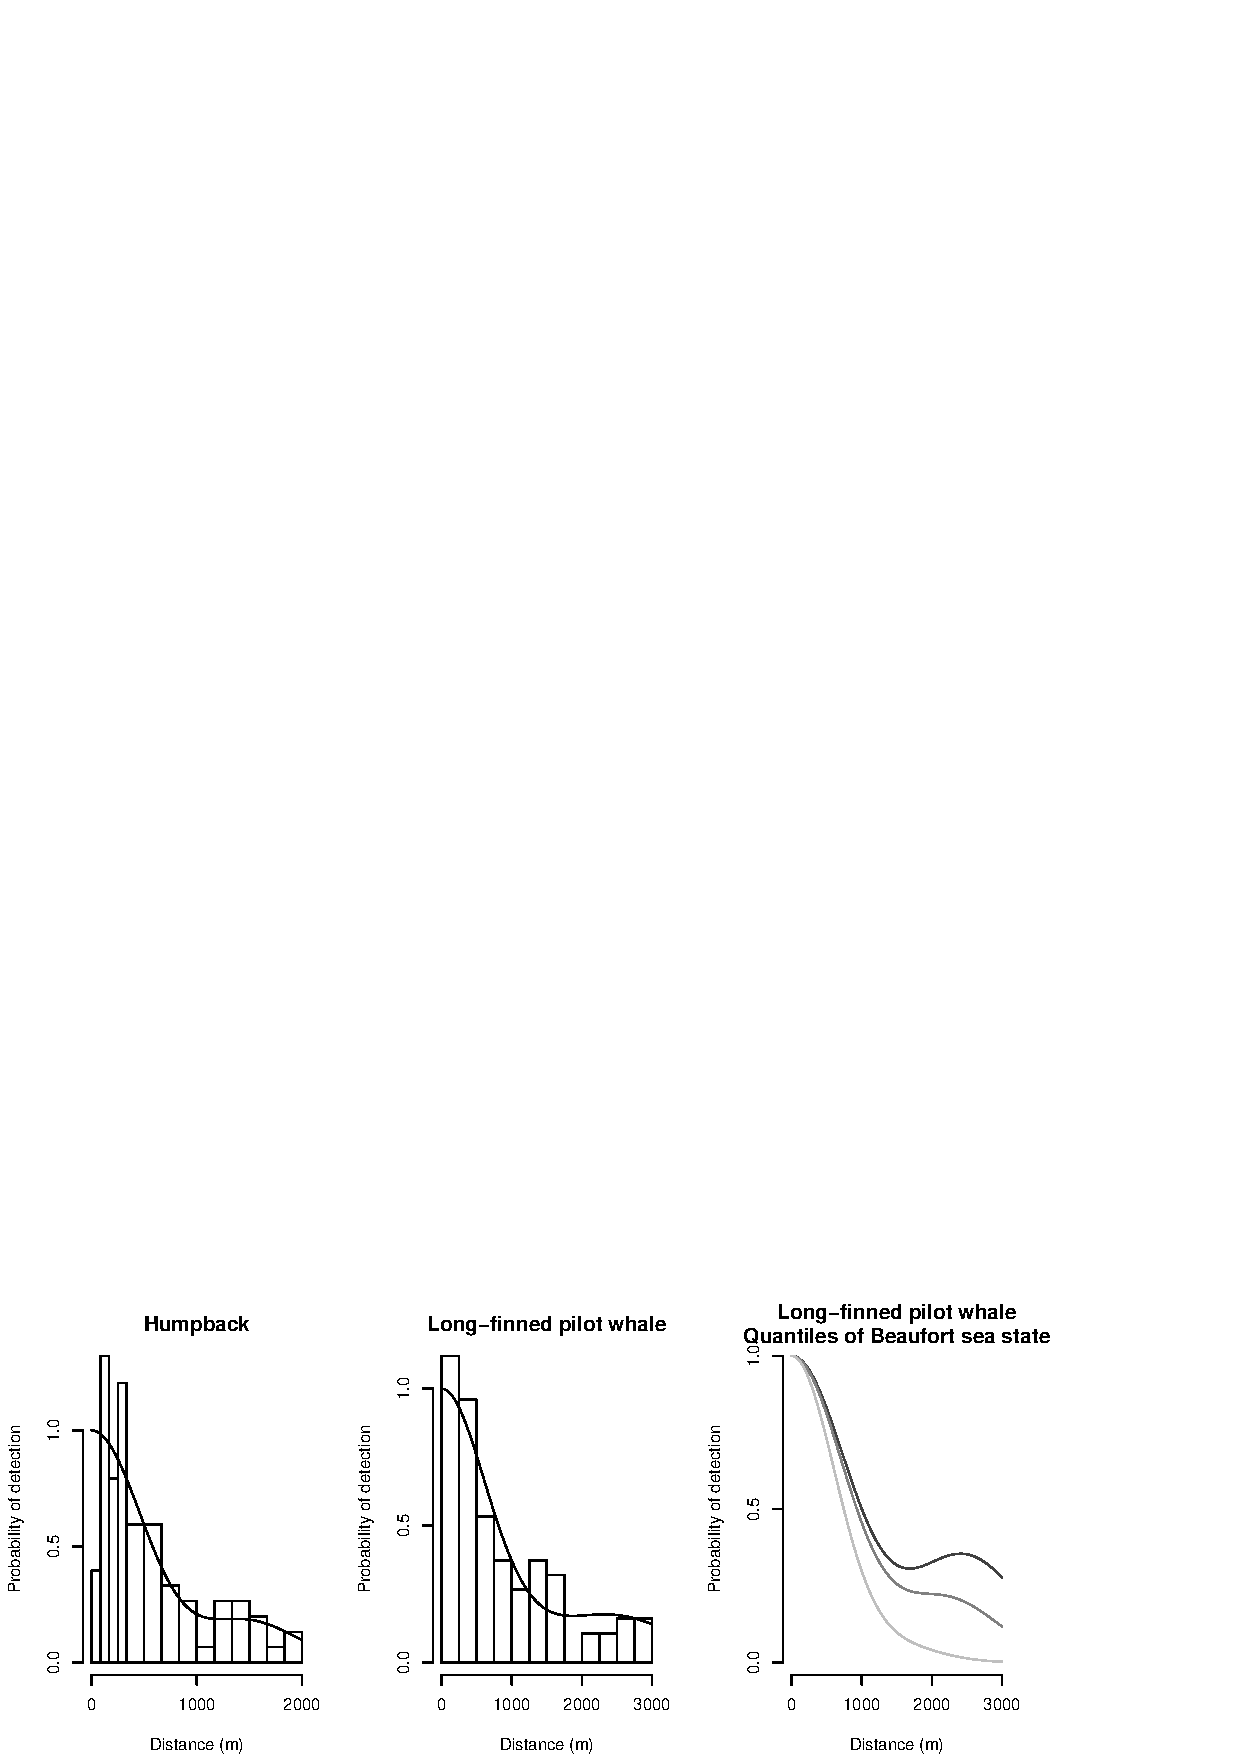
\includegraphics[width=\textwidth]{figs/figure1.pdf}
\caption{Two examples of detection functions that are not monotone, fitted using conventional key function plus adjustment methods in the software Distance. The left panel shows data from humpback whale \citep{Williams:2007tc}: a half-normal detection function with cosine adjustments was selected by AIC but even with constraints in place the detection function is non-monotonic, with a small secondary peak at approx. 1500m. The second and third panels show data and models fitted to long-finned pilot whale \citep{Pike:2003ug} where a half-normal detection function was selected with cosine adjustments and Beaufort sea state as a covariate. Due to the inclusion of covariates, no monotonicity constraints could be employed.  The middle panel shows the detection function averaged over the covariate values and the left panel the marginal detection function for 25th, 50th and 75th quantiles of the Beaufort sea state covariate; non-monotonicity occurs at approx. 2500m.}
\label{fig1}
\end{figure}

Mixture models have been applied in the capture-recapture literature following the work of \cite{Pledger:2000tc}, \cite{Dorazio:2003uf}, \cite{Pledger:2005wy} and \cite{Morgan:2008wy}. Their main utility in capture-recapture is in better accounting for between-individual heterogeneity, which can cause severe bias if unmodelled \citep{Link:2003wo}. Unmodelled heterogeneity is not generally considered an issue in distance sampling, provided that detection at zero distance is certain, heterogeneity is not extreme and a flexible detection function model is used \citep[][Section 11.12]{Buckland:2004ts}. Mixture models offer the potential for flexible modelling since the individual parts of the mixture model (the \textit{mixture components}) can be combined in various ways to yield a great many possible shapes, and yet all of these will be monotonic non-increasing so long as each component is monotonic non-increasing. In addition, mixture models are potentially well suited to deal with cases of high heterogeneity -- for example where some part of the population  is only observable at close distances while others are readily detected almost regardless of distance. Such a situation results in a ``spiked'' detection function with a long flat tail -- Figure \ref{fig1} shows relatively mild examples. In a mixture model, different parts of the sample could be represented by different components, providing a good fit to spiked data. 

In this paper, we introduce a new class of distance sampling detection function models, based on mixtures of simple parametric key functions.  In the next section, we describe the models.  We then illustrate their use and explore their performance by applying them to simulated data in Section 3, and to real data from a number of studies in Section 4. We also compare results with those obtained from the current standard key function and adjustment terms (K+A) approach, and by using a combined approach where both the mixtures and K+A models are applied and a final model selected using AIC.  We finish in Section 5 with a discussion of the utility of the new methods.  An R \citep{Team:2013wf} package, \texttt{mmds} (for Mixture Model Distance Sampling), implementing the methods is available from the Comprehensive R Archive Network (CRAN).

\section{Finite mixture model detection functions}

\subsection{Formulation}
\label{s:detfcts}

Denoting the detection function as $g$, we consider a sum of $J$ mixture components $g_j$, scaled by some mixture proportions $\phi_j$:
\begin{equation*}
g(y,\mathbf{z}; \bm{\theta}, \bm{\phi}) = \sum_{j=1}^J \phi_j g_j(y,\mathbf{z}; \bm{\theta}_j),
\end{equation*}
where $\sum_{j=1}^J \phi_j = 1$. The (radial or perpendicular) distance is denoted $y$, the $\bm{\theta}_j$s are vectors of parameters for function $g_j$, $\bm{\theta}$ is a vector of all of the $\bm{\theta}_j$s, $\bm{\phi}$ is a $J$-vector of all of the $\phi_j$s, and $\mathbf{z}$ is a $K$-vector of the associated covariates.  

Here we let the $g_j$s be half-normal functions (although other monotonic functions such as hazard-rate could be chosen and the $g_j$s need not all have the same form), so
\begin{equation*}
g(y,\mathbf{z}; \bm{\theta}, \bm{\phi}) = \sum_{j=1}^J \phi_j \exp \Big( - \frac{y^2}{2\sigma_j^2} \Big).
\end{equation*}
We assume that each mixture component has a different scale but that the covariates affect the scale parameters in the same way (though other, more complex, models may be possible).

Covariates are included as in \cite{Marques:2003vb}, by decomposing the scale parameter $\sigma$ \cite[see also][]{Marques:2007vm}.  Using $i$ to subscript each observation, our formulation for the scale parameter $\sigma_{ij}$, is
\begin{equation*}
\sigma_{ij} = \exp( \beta_{0j} + \sum_{k=1}^K \beta_k z_{ik}),
\end{equation*}
where $z_{ik}$ is the $k^\text{th}$ covariate for the $i^\text{th}$ observation. In this case $\bm{\theta}$ will contain the $\beta_{0j}$s and $\beta_k$s.

\subsection{Likelihood}
\label{s:likelihood}

As in \cite{Buckland:2004ts}, we can write the pdf of the observed distances conditional on the observed covariates as:
\begin{equation*}
f(y \vert \bm{z}; \bm{\theta}) = \frac{\pi(y)g(y, \bm{z}; \bm{\theta})}{\int_0^w \pi(y)g(y, \bm{z}; \bm{\theta}) \text{d}y}.
\end{equation*}
where $\pi(y)$ is the pdf of distances (observed and unobserved). The likelihood can then be formed by taking product of these pdfs over the $n$ observations.

For line transects, we denote a set of perpendicular distances to observations as $\{x_i; i=1,\ldots,n\}$ with associated covariate vectors $\{\bm{z}_i; i=1,\ldots,n\}$. With random line placement $\pi(x)=1/w$ (where $w$ is again the truncation distance). The likelihood is then given by:
\begin{align*}
\mathcal{L}(\bm{\theta},\bm{\phi}; \mathbf{x} \vert \bm{z}_1, \ldots, \bm{z}_n) &= \prod_{i=1}^n f(x_i \vert \bm{z}_i; \bm{\theta},\bm{\phi})\\
&= \prod_{i=1}^n \frac{g(x_i,\bm{z}_i; \bm{\theta},\bm{\phi})}{\mu_i(\bm{z}_i)}\\
&= \prod_{i=1}^n \frac{\sum_{j=1}^J \phi_j g_j(x_i,\bm{z}_i; \bm{\theta}_j)}{\mu_i(\bm{z}_i)}
\end{align*}
where $\mu_i(\bm{z}_i)$, the \textit{effective strip width}, is given by:
\begin{equation*}
\mu_{i}(\bm{z}_i) = \sum_{j=1}^J \phi_j \int_0^w  g_j(x,\bm{z}_i; \bm{\theta}_j) \text{d}x.
\end{equation*}

For point transects, denote radial distances $\{r_i; i=1,\ldots,n\}$ and associated covariate vectors $\{\bm{z}_i; i=1,\ldots,n\}$. With random point placement, $\pi(r)=2r/w$, the likelihood is then:
\begin{align*}
\mathcal{L}(\bm{\theta},\bm{\phi}; \mathbf{r}  \vert \bm{z}_1, \ldots, \bm{z}_n) &= \prod_{i=1}^n f(r_i \vert \bm{z}_i; \bm{\theta},\bm{\phi})\\
&= \prod_{i=1}^n \frac{2 \pi r_i g(r_i,\bm{z}_i; \bm{\theta},\bm{\phi})}{\nu_i}\\
&= \prod_{i=1}^n \frac{2 \pi r_i \sum_{j=1}^J \phi_j g_j(r_i,\bm{z}_i; \bm{\theta}_j)}{\nu_i}
\end{align*}
where the \textit{effective area of detection}, $\nu_i$ is defined as:
\begin{equation*}
\nu_i = 2\pi \sum_{j=1}^J \phi_j \int_0^w  r g_j(r,\bm{z}_i; \bm{\theta}_j) \text{d}r.
\end{equation*}

For both line and point transects, parameters are estimated using maximum likelihood. Practicalities associated with this maximization, along with analytic derivatives of the likelihood are described in Web Appendices A and B.

In this article, we have assumed that the distance data are in the form of ``exact'' distances from detected objects to the transect; alternatively, distances can be grouped into intervals, with pre-defined cutpoints (e.g., 0-10m, 10-20m, etc.), so that the data are the distance interval of each observation.  In this case, a multinomial likelihood is obtained \citep[see, e.g.][Section 3.3.2]{Buckland:2001vm}.

\subsection{Estimating population size}
\label{s:popsize}

Population size can be estimated using the Horvitz-Thompson-like estimator \citep{Marques:2003vb}:
\begin{equation}
\label{e:popsize}
\hat{N}=\frac{A}{a}\sum_{i=1}^n \frac{1}{\hat {p}_i}
\end{equation}
where $A$ is the area of the study region for which population size is being estimated, $a$ is the size of the sampled area, and $p_i$ is the probability of the $i^\text{th}$ observation being detected given it is within the sampled area.  For line transects, $a=2wL$ where $L$ is the total line length, and 
\begin{equation*}
p_i = \frac{1}{w} \sum_{j=1}^J \phi_j \int_0^w  g_j(x,\mathbf{Z}; \bm{\theta}_j) \text{d}x.
\end{equation*}
For point transects, $a=\pi w^2 k$ where $k$ is the number of points, and 
\begin{equation*}
p_i = \frac{2\pi}{w^2} \sum_{j=1}^J \phi_j \int_0^w  r g_j(r,\mathbf{Z}; \bm{\theta}_j) \text{d}r.
\end{equation*}
A standard summary statistic is the average detection probability for an animal within the sampled area, $P_a$, which is given by:
\begin{equation*}
P_a = n/N.
\end{equation*}
Estimators for the variances of $\hat{N}$ and $\hat{P_a}$ are given in Web Appendix C.

\section{Simulations}
\label{s:sims}

\subsection{Simulation methods}

Extensive simulations were carried out to investigate performance (in terms of the accuracy of estimation of $P_a$) when the true detection function model is not known to the estimation procedure.  

Each simulation involved generating 200 replicate datasets from a specified detection function model (assuming the entire study area was included within the surveyed transects, i.e., $A=a$ in equation (\ref{e:popsize}), and a truncation distance of $w=1$), fitting each dataset with a range of mixture and key series plus adjustment term (K+A) models, and in each case recording estimated parameter values and abundance from the model with the lowest AIC in each of: mixture models, K+A models, and both combined.  Mixture models with 1-, 2-, and 3-point half-normal components were fitted to the data along with two K+A models: half-normal plus cosine adjustments and hazard rate plus simple polynomial adjustments, both with monotonicity constraints implemented as described above and with a maximum of 3 adjustments. Mixture models and K+A models were fitted using the R packages \texttt{mmds} (version 1.1) and \texttt{Distance} (version 0.6.1) respectively, both written by the authors.

Fourteen different simulation scenarios were investigated, in five groups, as described below and illustrated in Figure \ref{sim-detfcts} (one line per group). (True parameter values are given in Web Appendix D.)  For each scenario, a simulation was performed at each of five sample sizes (number of observations): 30 (low), 60 \citep[recommended minimum for line transects;][]{Buckland:2001vm}, 120 (adequate), 480 (large) and 960 (very large).  We anticipated performance would depend upon sample size, because: the methods are likelihood-based and hence only asymptotically unbiased even if the correct model is fitted; the use of AIC to select model complexity meant that more flexible (and hence accurate) models could be expected to be selected given larger sample sizes; mixture models are ``parameter hungry'' compared with K+A models (in the sense that each additional mixture component requires 2 extra parameters, while each additional adjustment term requires only one) and hence, given the use of AIC for model selection, the relative performance of the two approaches may change at different sample sizes. We now list the five simulation scenario groups.


\begin{figure}
\centering
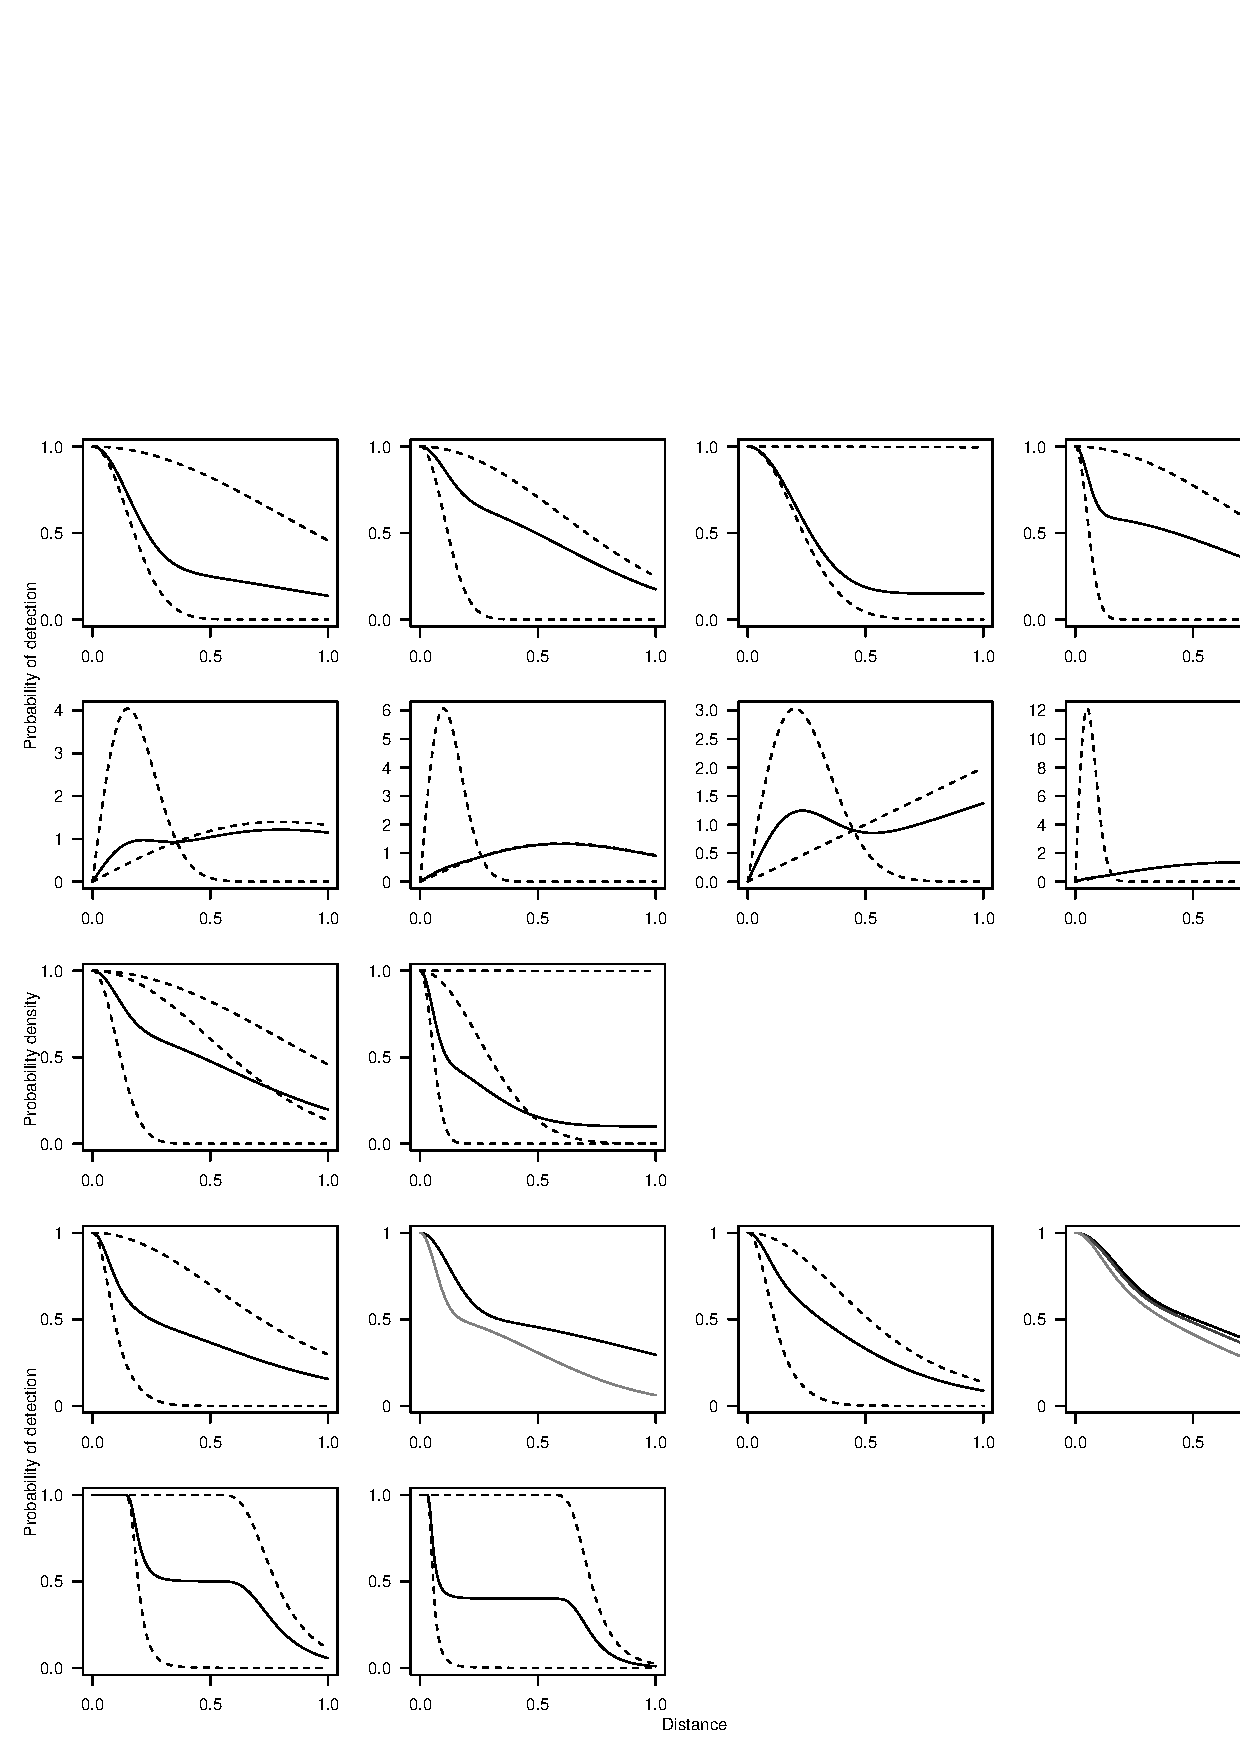
\includegraphics[width=\textwidth]{figs/sim-detfct.pdf}
\caption{Plots of the models used in the simulation. Group A (top row): detection functions for four line transect senarios with no covariates (solid lines) and their constituent mixture components (dashed lines). Group B (second row): pdfs for four point transect simulations with no covariates (solid lines), with associates component pdfs (dashed lines), rescaled so the area under each curve is one; the detection functions are as in the top row. Group C (third row): two 3-point mixture scenarios for non-covariate line transect data. Group D (fourth row): two covariate model scenarios, the first two panels are for a binary covariate scenario, the second two for a continuous covariate scenario; first panels in each pair show the detection function averaged over the covariates (along with the mixture components, similarly averaged) and the second panels show marginal detection functions with the levels (or quantiles) of the detection function.  Group E (fifth row): detection functions for two line transect scenarios using 2-point mixtures of hazard rate functions.}
\label{sim-detfcts}
\end{figure}

\textit{Group A. Line transect with 2-point half-normal mixture detection functions.} Four scenarios were tested, representing a range of potentially challenging detection functions.  Scenarios A1 and A2 both have mixture components with quite different scale parameters, but in A1 the majority of data come from the less detectable component while in A2 it comes from the more detectable component.  A3 tests the behaviour of the models when the scale parameter of one of the mixture components is very large relative to the truncation distance. A4 has a large spike (i.e., a sharp decline in detectability at small distances), which is similar to some of the data we analyse in Section \ref{s:data}.

\textit{Group B. Point transect with detection functions as in the previous scenario.} The geometry of point transect sampling means there are few animals close to the point relative to those at larger distances. Hence there are few observations that are only detectable at smaller distances, even though these animals make up a significant proportion of the population. We therefore anticipate that performance will be worse for point transects. For this group, Figure \ref{sim-detfcts} shows pdfs of the observed distances.

\textit{Group C. Line transect with 3-point half-normal detection functions.} Two scenarios were tested. C1 has a detection function much like A2, enabling us to investigate the efficacy of model selection (i.e., we expect a 2-point mixture to be selected and to produce good results). C2 is a more complex shape that could only be created using a 3-point mixture; it has the added complication (as with A3) that one of the components has a large scale parameter relative to truncation distance.

\textit{Group D. Line transect with 2-point half-normal detection functions with additional covariates.}  We used covariate models to test two aspects of model robustness. In the first, we assumed the covariate values were observed, and included multiple covariate models in the candidate set, along with distance-only models. Our prediction was that (at large sample sizes at least) multiple covariate models would be selected and estimation of $P_a$ unbiased.  In the second, we assumed the covariate values were not observed, and hence multiple covariate models were not in the candidate set.  Our expectation was that (at larger sample sizes) more complex mixture distributions would be selected to compensate for the additional unobserved complexity, and that estimation of $P_a$ would not be greatly affected.  Two scenarios were tested.  D1 had a binary factor covariate, with half the observations having one covariate value and half the other.  D2 had a continuous covariate, whose values were generated from a standard normal distribution function.  Detection functions are shown in the fourth row of Figure \ref{sim-detfcts}, along with the marginal detection functions for the levels/quantiles of the covariates. Note that, for the unobserved covariate models, D1 is equivalent to a 4-point mixture, while D2 is equivalent to a 2-point continuous mixture; neither of these models were in the candidate model set.  

\textit{Group E. Line transect with 2-point hazard rate mixture detection functions.} The above models all use the same functional form for $g_j$ in generation and fitting. So mixtures of hazard-rate functions were used to generate observations where the true model was not in the candidate set (see Web Appendix D for formulation). E1 has a shape that may be difficult to fit with half-normal models; E2 has the added complication of a severe spike in detectability at small distances.
  
\subsection{Simulation results}
\label{s:sims_res}

Figure \ref{sim-boxplots} summarizes the estimates of $P_a$ obtained if only mixture models (including 1-point mixtures) are included in the candidate model set (i.e., excluding the K+A models); the numbers below each boxplot are the proportion of times the correct model was selected.  Web Appendix E shows the distribution of estimates when only K+A models are used (giving a baseline to compare the mixture model results against, Web Figure 2), the distribution of estimates when both mixture and K+A models are included (which might be a recommended modelling strategy, Web Figure 3), and the proportion of time each model is chosen using the combined modelling strategy (Web Figure 4).

\begin{figure}
\centering
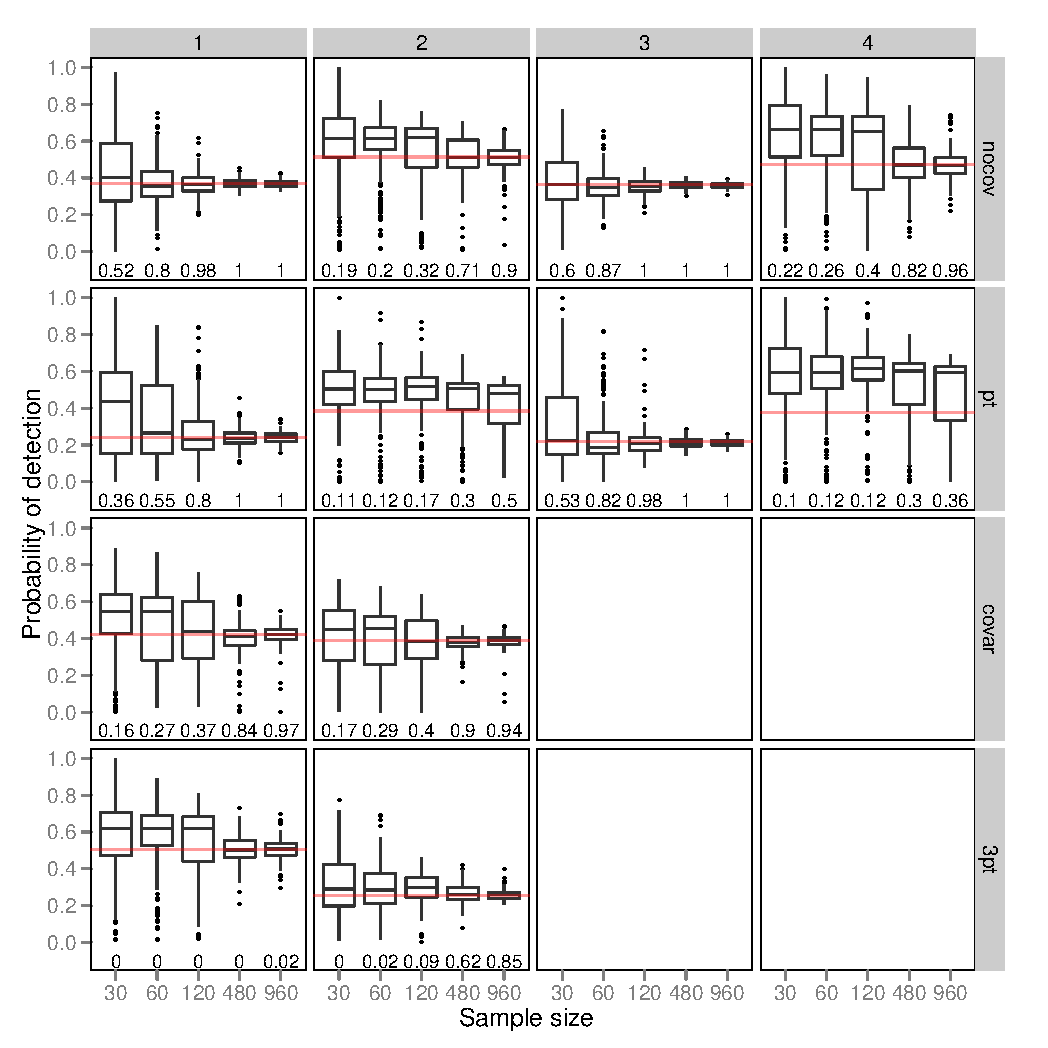
\includegraphics[width=\textwidth]{simulations/pa-plot.pdf}
\caption{Simulation results: boxplots of the estimated average detection probabilities, $P_a$, for the best model (by AIC score). Layout is as in Figure \ref{sim-detfcts}. Grey lines indicate the true value of the average detection probability. Numbers underneath each boxplot give the proportion of AIC best models that were of the same form as the model that the data was simulated from (e.g., in covariate scenario 1 the proportion of AIC best models that were 2-point mixtures that included the covariate in the model).}
\label{sim-boxplots}
\end{figure}

For Group A, the mixture approach produced unbiased results for scenarios A1 and A3, even at very low sample sizes, and even though the correct 2-point mixture model was selected only 50-60\% of the time at the lowest sample size (Figure \ref{sim-boxplots}; the half normal model was selected the remainder of the time).  The K+A approach also performed well (Web Figure 2). Unsurprisingly, therefore, the combined approach performed well (Web Figure 3); what was a little surprising was that the correct model was only selected 60-76\% of the time at the highest sample sizes for scenario A1, with the hazard-rate K+A model selected the remainder (Web Figure 4). This emphasizes the utility of flexible modelling approaches. Scenarios A2 and A4 showed positive bias at smaller sample sizes under the mixture approach; bias reduced substantially by 480 observations, where a large proportion of the selected models were 2-point mixtures. Unlike scenarios A1 and A3, the detection functions in scenarios A2 and A4 were evidently not well approximated by a half-normal. The K+A approach did not fare well with these scenarios, showing strong positive bias even at large sample sizes. In combination, the mixture models were chosen over K+A models at larger sample sizes, and so the combined modelling approach produced much better results than K+A alone.  

As expected, results were worse for the point transect scenarios of Group B.  Estimates from the mixture approach were slightly biased at low sample sizes for B1, when the two-point model was rarely selected, but were unbiased given 120 observations and greater.  Estimates for B3 were unbiased.  For B2 and B4, results were positively biased at small sample sizes, just as with A2 and A4, but unlike the line transect scenarios the bias did not disappear even at the largest sample size.  This is unsurprising given the very small number of detections coming from the less detectable mixture component (see Figure \ref{sim-detfcts} -- the marginal pdf is almost identical to that of the easier to detect mixture component). Despite this, bias was generally worse with the K+A approach (Web Figure 2), and the combined approach (Web Figure 3) produced marginally better results than K+A alone; for scenario B3 the combined results were much better. 

Group C were the 3-point mixture scenarios.  For C1, results were similar to A2 -- unsurprising, given the similarity in detection functions.  A 3-point mixture model was almost never chosen by AIC (Figure \ref{sim-boxplots}).  For C2, estimates were surprisingly good, even when the 3-point mixture was not the selected model, at lower sample sizes.  In both cases, the K+A results were worse (Web Figure 2), and the combined results were as good as those using mixtures alone (Web Figure 3).

We first address the results of the Group D simulations when covariates were available for inclusion in candidate models. In this case, results are positively biased at lower sample sizes but as sample size increases the true probability of detection is found. The K+A models are generally positively biased, though with less variation (Web Figure 2), where as the combined result gives the best of both of these worlds. When covariate information is not available for fitting the model, the mixture model detection functions still perform well, showing that when covariates are not available mixture components can compensate.

The Group E results, simulated using mixtures of hazard-rate functions, were a little disappointing.  The half-normal mixture models produced a small positive bias in all cases, except for larger sample sizes in scenario E1, where the bias was negative.  The K+A models had similar (for low sample size) or lower (for high sample size) bias in E1, but higher bias in E2, and the combined approach showed little improvement in performance over K+A alone.

\section{Case studies}
\label{s:data}

The first two case studies return to the datasets depicted in Figure \ref{fig1}, and demonstrate how the mixture formulation solves the issue of non-monotonic detection functions.  The first case study also includes two other species, illustrating how the new approach can fit real data as well as, or better than, the K+A approach.  The third case study demonstrates modelling of spiked line transect data, while the fourth gives a point transect example.

\subsection{British Columbia marine mammals}

\cite{Williams:2007tc} used a data from a line transect survey to study several species of marine mammal off the coast of British Columbia, Canada. Here, we investigate three species: harbour seal (\textit{Phoca vitulina}) in water, harbour porpoise (\textit{Phocoena phocoena}) and humpback whale (\textit{Megaptera novaeangliae}). Truncation distances were set at 500m, 500m and 2000m for each species respectively, giving sample sizes of 232, 59, and 70 observations. Results are summarised in Table \ref{williams-pike-table} and detection functions for the AIC-best models are shown in Figure \ref{williams-detfcts}.

Two-point mixture models were selected for all species.  For harbour seal, the mixture model had a lower AIC and better goodness-of-fit $p$-value than for the K+A model of \cite{Williams:2007tc}.  The $\hat{P}_a$ is approximately 20\% lower, implying that the previous estimate of $\hat{N}$ may have been an overestimate.  For harbour porpoise, the mixture model AIC is almost 2 points higher than the K+A model, which was a hazard-rate with no adjustments.  Hence, the model deviances are very similar, but the penalty due to the 2-point mixture having an additional parameter prevents it from being selected.  The $\hat{P}_a$ from the two models are very close.  Lastly, for humpback whales, the mixture model AIC is almost 3 points higher than the K+A model -- however, one advantage of the mixture model is that the fitted function is monotone (Figure \ref{williams-detfcts}) while the K+A function is not (Figure \ref{fig1}).  Again, the estimated $\hat{P}_a$s are very similar.

\begin{figure}
\centering
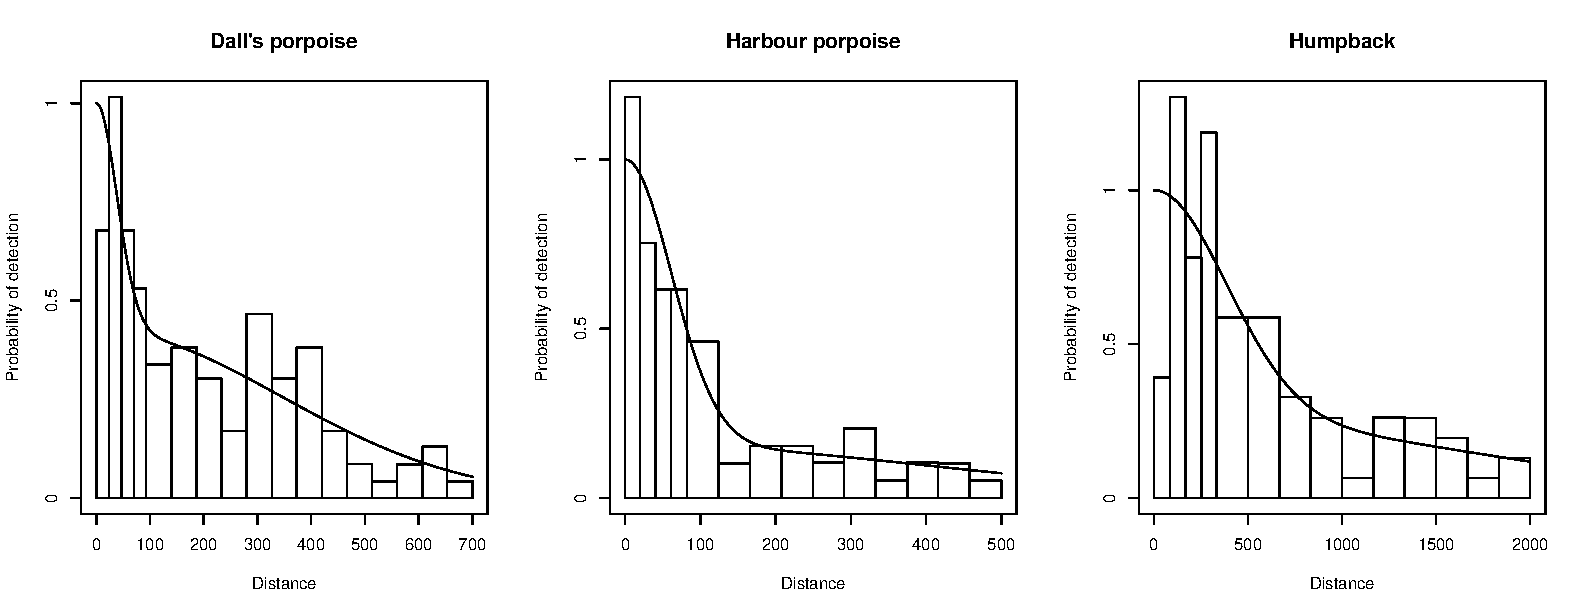
\includegraphics[width=\textwidth]{analyses/williamsplots.pdf}
\caption{Plots of the mixture model detection functions fit to the British Columbia marine mammal data. In each case the best model by AIC was a 2-point mixture. Dashed lines show the mixture components.}
\label{williams-detfcts}
\end{figure}

\subsection{Long-finned pilot whales}

\cite{Pike:2003ug} analyzed observations of 84 pods of long-finned pilot whales (\textit{Globicephala melas}), sighted as part of a line transect survey, the North Atlantic Sightings Survey NASS-2001. The Beaufort sea state was recorded as a covariate during the survey and enters the authors' model as either a continuous variable, or a factor with 2, 3, or 6 levels.

A mixture model detection function was fitted with each of these covariates, as well as a model with no covariates.  The best model by AIC score (Table \ref{williams-pike-table}) was a 2-point mixture with Beaufort sea state included as a continuous covariate. Figure \ref{danpike-detfct} shows the average detection function (in the sense that a detection function fitted to each covariate combination was evaluated over the range $(0,w)$ and then averaged point-wise) and the marginal detection function with the quantiles of Beaufort sea state. As one would expect, none of the non-monotonic behaviour seen in Figure \ref{fig1} can be seen here.

\begin{figure}
\centering
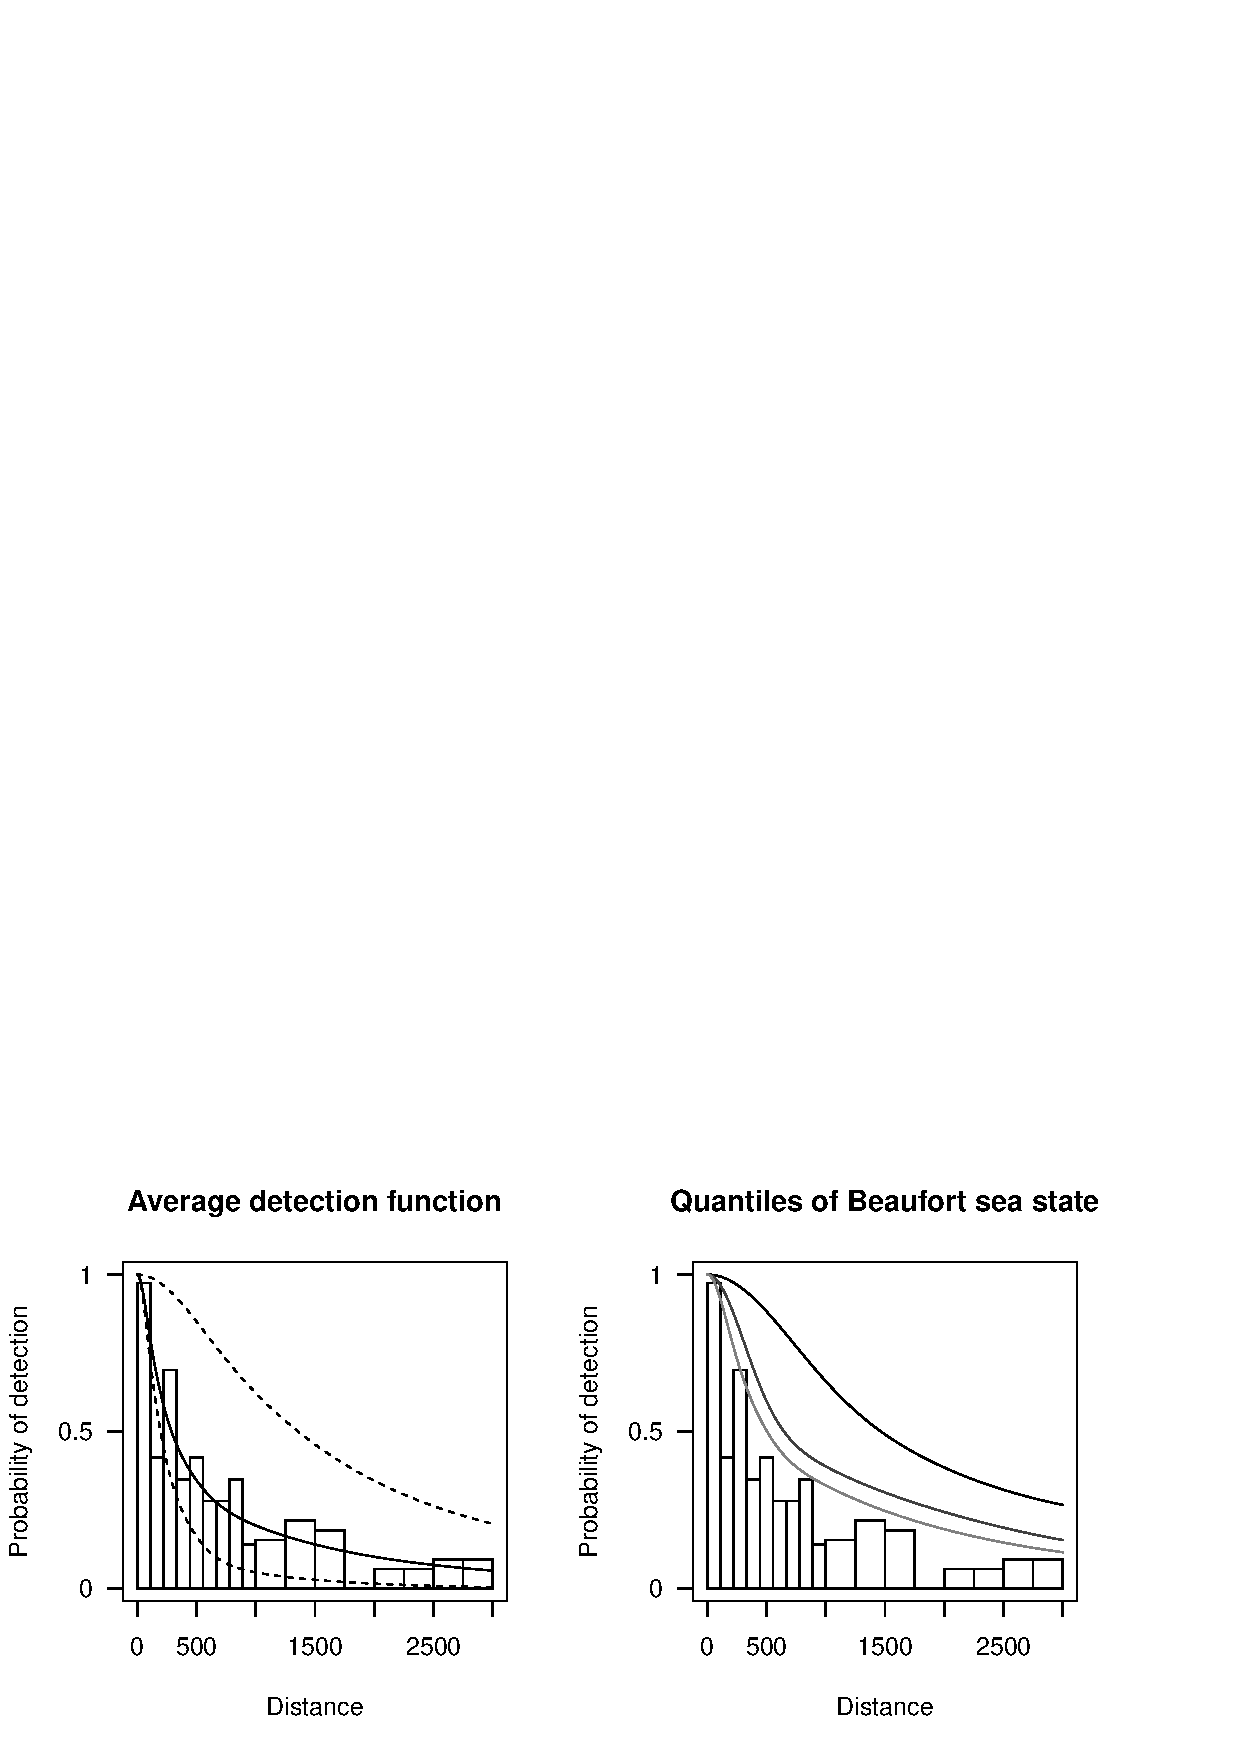
\includegraphics[width=0.375\textwidth, trim= 0 0 3.8in 0, clip=true]{analyses/danpike-bssc.pdf}\includegraphics[width=0.375\textwidth, trim= 3.8in 0 0 0, clip=true]{analyses/danpike-bssc-hh.pdf}
\caption{The (AIC) best model for the long-finned pilot whale data: a 2-point mixture model detection function with Beaufort sea state as a continuous covariate. Left: the average detection function with components as dashed lines. Right: the marginal detection function with the quantiles (25\%, 50\% and 75\%) of the Beaufort sea state.}
\label{danpike-detfct}
\end{figure}


\subsection{Wood ants}
\label{s:woodant}

\cite{Borkin:2012wn} analyse data on two species of wood ant (\textit{Formica aquilonia} and \textit{Formica lugubris}) collected during a line transect survey of the Abernethy Forest, Scotland, in 2003. The number of nests sighted was 150 out to a distance of 72.04m from the track line, although 45\% of the nest sightings lay within 4m of the line. As part of their analysis, several different truncation distances were used. Larger truncation distances led to a large variance in the encounter rate estimates and hence in overall abundance estimates \citep[see][]{Borkin:2012wn}. This is due to the spike caused by the large number of detections close to the line (see Web Figure 5).

As well as distances, three covariates were recorded: habitat type (a four level factor), the size of each nest (a continuous variable, calculated as half-width multiplied by height) and species (a two level factor). All combinations of main effects were fit (Web Table 2), and the best model by AIC was a 2-point mixture with nest size and habitat as covariates (Web Figure 5). This model had an AIC that was considerably lower (6 points) than the AIC-best K+A model, a hazard-rate with the same covariates.  The estimated $P_a$ is about 10\% lower with the mixture model.

\subsection{Amakihi}
\label{s:amakihi}

\cite{Marques:2007vm} analyse point transect data on a Hawaiian songbird, the Amakihi (\textit{Hemignathus virens}). The data consist of 1243 observations (after truncation at 82.5m), collected at 41 points between 1992 and 1995, together with three covariates in addition to distance: the observer (a three level factor), minutes after sunrise (continuous) and hours after sunrise (a six level factor).

The AIC-best mixture model was a two point mixture with observer and minutes after sunrise as covariates (shown in Web Figure 6), closely followed by the model with only observer as a covariate (Web Table 2). In this case a hazard-rate with observer and minutes after sunrise as covariates beat the mixtures in AIC terms. This is not too surprising given that the mixtures use one more parameter than a hazard-rate in this situation. It is encouraging that there is such a small difference in AIC, and that covariate mixture models were selected despite the large number of parameters that such models entail.

\begin{table}
\caption[]{Comparison of results from \protect{\cite{Williams:2007tc}}, \protect{\cite{Pike:2003ug}}, \protect{\cite{Borkin:2012wn}} and \protect{\cite{Marques:2007vm}} with results from fitting mixture model detection functions. In each case the first line for each data set is the model from the original article. Mixture model components were selected by AIC. In each case the AIC-best model is emboldened, but note for the \protect{\cite{Williams:2007tc}} data, all models were close in AIC terms. In the table ``(cont.)'' denotes that the covariate was included in the model as continuous, otherwise covariates entered the model as factors (\texttt{BBSn} indicates Beaufort sea state with \texttt{n} factors). $\cos(x)$ indicates a Cosine adjustment of order $x$. }
\centering
\begin{tabular}{c c c c c c}
\hline \hline
Species & Model & AIC & $\hat{P_a}$ & $\% CV \hat{P_a}$ & K-S $p$\\
\hline
Harbour seal & Hn+$\cos(2)$ & 2771.05 & 0.425 & 7.55 & 0.515\\
(in water) & Hn 2-pt  & \textbf{2769.86} & 0.335 & 15.38 & 0.945\\
&&&&&\\
Harbour & Hr  & \textbf{690.66} & 0.212 & 32.0 & 0.99\\
porpoise & Hn 2-pt & 692.09 & 0.254 & 18.18 & 0.99\\
&&&&&\\
Humpback & Hn+$\cos(2)$ & \textbf{1033.06} & 0.386 & 12.64 & 0.672 \\
whale & Hn 2-pt & 1035.94 & 0.381 & 18.48 & 0.649 \\
&&&&&\\
Long-finned & Hn 1-pt + $\cos(2)$ \texttt{BSS} (cont.) & 1286.5 & 0.452 & 8.69 & 0.48\\ % mrds
% Hn 1-pt + $\cos(2)$& \texttt{BSS} (cont.) & 1296 & 0.37 & 9.56 & 0.319 \\ % Distance result 
pilot whales  & Hn 2-pt &  1298.42  &  0.295  &  17.17  &  0.95 \\
 & Hn 2-pt \texttt{BSS6} &  1286.26  &  0.152  &  670.93  &  0.83 \\
 & Hn 2-pt  \texttt{BSS2}  &  1284.99  &  0.211  &  23.39  &  0.95 \\
 & Hn 2-pt  \texttt{BSS3}  &  1296.27  &  0.27  &  17.46  &  0.99 \\
 & Hn 2-pt  \texttt{BSS} (cont.) &  \textbf{1284.56}  &  0.216  &  24.17  &  0.67 \\
 &&&&&\\
Wood ants & Hn 2-pt  None  &  754.61  &  0.184  &  15.46  &  0.96 \\
 & Hn 2-pt \texttt{habitat} &  751.27  &  0.188  &  14.85  &  0.97 \\
 & Hn 2-pt \texttt{species} &  756.59  &  0.184  &  15.48  &  0.94 \\
 & Hn 2-pt \texttt{nest.size} &  741.64  &  0.214  &  15.19  &  0.76 \\
 & Hn 2-pt \texttt{habitat} + \texttt{species} &  753.23  &  0.186  &  14.94  &  0.99 \\
 & Hn 2-pt \texttt{habitat} + \texttt{nest.size}  &  \textbf{737.27}  &  0.179  &  17.55  &  0.72 \\
 & Hn 2-pt \texttt{nest.size} + \texttt{species}   &  741.92  &  0.21  &  15.84  &  0.77 \\
 & Hn 2-pt \texttt{nest.size} + \texttt{species} + \texttt{habitat}  &  739.08  &  0.178  &  18.09  &  0.83 \\
% & Hr  \texttt{nest.size} + \texttt{habitat} & 745.2 & 0.194 & 10.6 & 0.95\\  % Distance result 
 & Hr \texttt{nest.size} + \texttt{habitat} & 743.56 & 0.195  & 21.72 & 0.89\\ % mrds result
 &&&&&\\
Amakihi & Hn 2-pt &  10805.48  &  0.283  &  6.21  &  0.12 \\
 & Hn 2-pt \texttt{obs} &  10778.69  &  0.279  &  5.86  &  0.04 \\
 & Hn 2-pt \texttt{has}  &  10807.19  &  0.282  &  6.95  &  0.33 \\
 & Hn 2-pt \texttt{mas}  &  10805.11  &  0.284  &  6.52  &  0.31 \\
 & Hn 2-pt \texttt{obs} +\texttt{has}  &  10782.53  &  0.283  &  6.21  &  0.23 \\
 & Hn 2-pt \texttt{obs} +\texttt{mas}  &  10778.07  &  0.279  &  6.1  &  0.14 \\
 & Hn 2-pt \texttt{mas} +\texttt{has}  &  10809.17  &  0.282  &  6.97  &  0.43 \\
 & Hn 2-pt \texttt{mas} +\texttt{has}+\texttt{obs}  &  10784.5  &  0.282  &  6.33  &  0.35 \\
%  &  Hr & \texttt{obs} + \texttt{mas} & \textbf{10777.72} & 0.3 & 2.65 & 0.036 \\ % Distance result 
 & Hr \texttt{obs} + \texttt{mas} & \textbf{10777.38} &  0.319 & 5.11 & 0.076\\ % mrds
\hline
\end{tabular}
\label{williams-pike-table}
\end{table}

\section{Discussion}
\label{s:discuss}

[Conclusion - works well fof some types of spiked data. - -may help.]
[Discuss fitting strategy - combined approach]

[Simulation study showed that:
This group demonstrates that the mixture approach can have practical advantages over the K+A approach, either when used as an alternative or as part of a combined model selection strategy, and particularly for some kinds of spiked data.
Can also have advantages for point transect data, but no approach is well able to cope with a spike there.]

We have investigated and demonstrated the utility of detection functions constructed from mixtures of half-normals in both line and point transect distance sampling. We also show that covariates can be included in such models easily. These mixture detection functions can be simply ``dropped into'' existing models such as: methods for dealing with incomplete detection at zero distance \citep{Laake:2004tz, Laake:2011vm} or spatial models for distance sampling data \citep{Hedley:2004et, Miller:2013us}.

We have shown that the method performs well on both simulated and case studies where traditional methods produce unrealistic results. In many cases the proposed model outperformed K+A models in AIC terms, which is surprising given that the mixture models in question often had more parameters. 

Simulations show that small sample sizes do not support the use of mixture models with a high number of components, even when the data were generated from such a model. We avoid poorly fitting models of this sort by using both K+A and mixture detection functions and selecting the best between them (comparing Fig. \ref{sim-boxplots} with Web Figure 2). This integrated approach is not dissimilar to current model selection procedures for a detection function analysis -- currently selection is made between different K+A formulations (and number of adjustment terms) using AIC, mixture models simply add another alternative detection function where rather than adjustment terms, mixture components are selected.

In simulation we observed that 3-point mixture did not act as good surrogates for missing covariate information; 2-point mixtures were generally chosen by AIC as good models.  In Section \ref{s:data}, 2-point mixtures consistently provided the best fit. Only examination of further data will show whether 3-point and higher mixtures can be supported, however we note that when the K$+$A series formulation is used, detection functions with 5 or more parameters are rarely selected by AIC (a 3-point mixture with no covariates requires 5 parameters).

All the models discussed in this article are available as an \textsf{R} package, \texttt{mmds} which is available on CRAN. Mixture model detection functions will be available in the next version of the Distance software and the \textsf{R} package \texttt{Distance}.

Further work will include extending these models further to include continuous mixtures. In that case the detection function can be modelled as:
\begin{equation*}
g(x) = \int_\mathbf{R} \varphi(\kappa) g_\kappa(x,\mathbf{Z}; \theta, \kappa) \text{d}\kappa
\end{equation*}
where $\varphi(\kappa)$ is a weighting function which controls the mixing of $g_\kappa$. Such an approach may present significant computational issues, however the benefits of a significantly more flexible detection function may be considerable. Provided that an appropriate function can be chosen for $\varphi$, more flexible models could be used whilst keeping the number of parameters low. In addition, a combination of both finite and continuous mixtures could be used, echoing the work of \cite{Morgan:2008wy} in capture-recapture.

\backmatter

%  This section is optional.  Here is where you will want to cite
%  grants, people who helped with the paper, etc.  But keep it short!

\section*{Supplementary material}

Web Appendices referenced in Sections \ref{s:likelihood}, \ref{s:popsize}, \ref{s:sims_res}, \ref{s:woodant} and \ref{s:amakihi} are available with this paper at the Biometrics website on Wiley Online Library.

\section*{Acknowledgements}

DLM acknowledges the UK EPSRC for financial support, and Simon Wood for useful discussions.  Both authors thank David Borchers, who suggested the parametrisation for the mixture proportions (Web Appendix A), as well as the following people, who provided case study data: Rob Williams (B.C. marine mammals), Dan Pike (pilot whales), Kelly Borkin (wood ants) and Steve Fancy (Amakihi).

\bibliographystyle{chicago}
\bibliography{dsmixtures}

\label{lastpage}

\end{document}